\documentclass[tikz,border=4pt]{standalone}
\usepackage{tikz}
\usepackage{amsmath}
\usetikzlibrary{arrows.meta,calc,positioning,shapes.geometric,patterns,backgrounds,fit}

\begin{document}
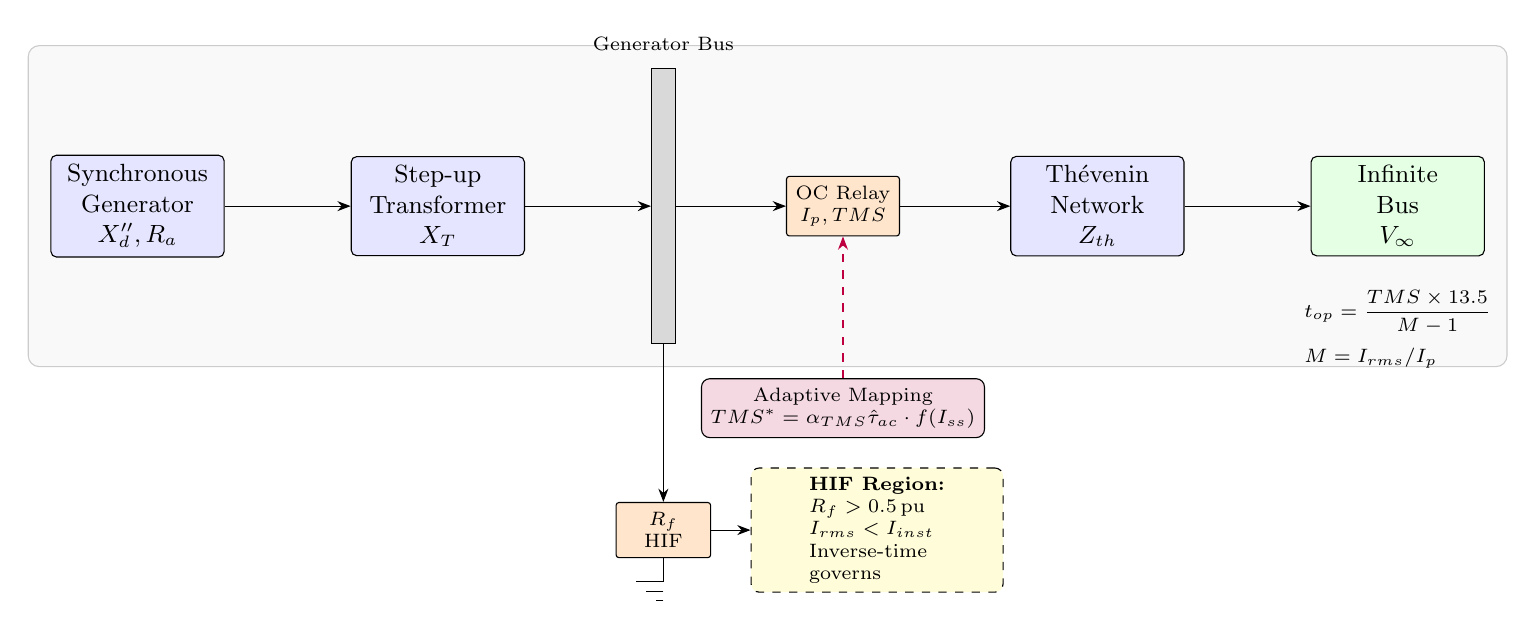
\begin{tikzpicture}[
  font=\small,
  >=Stealth,
  bus/.style ={draw,rectangle,fill=gray!30,minimum width=0.3cm,minimum height=3.5cm},
  box/.style ={draw,rectangle,fill=blue!10,minimum width=2.2cm,minimum height=0.9cm,
               align=center,rounded corners=2pt},
  relay/.style={draw,rectangle,fill=orange!20,minimum width=1.2cm,minimum height=0.7cm,
                align=center,font=\scriptsize,rounded corners=1pt},
  ground/.style={},
]

%% =============================================
%% Generator on left
%% =============================================
\node[box] (gen) at (0,0) {Synchronous\\Generator\\$X_d'',R_a$};

% Step-up transformer
\node[box,right=1.6cm of gen] (xfmr) {Step-up\\Transformer\\$X_T$};

%% =============================================
%% Generator bus
%% =============================================
\node[bus,right=1.6cm of xfmr] (gbus) {};
\node[above=0.1cm of gbus,font=\scriptsize] {Generator Bus};

%% =============================================
%% Relay on feeder out of bus
%% =============================================
\node[relay,right=1.4cm of gbus] (relay) {OC Relay\\$I_p,TMS$};

%% =============================================
%% Thevenin network
%% =============================================
\node[box,right=1.4cm of relay] (zth) {Th\'{e}venin\\Network\\$Z_{th}$};

% Infinite bus
\node[box,right=1.6cm of zth,fill=green!10] (infbus) {Infinite\\Bus\\$V_\infty$};

%% =============================================
%% Fault branch (drops down from bus)
%% =============================================
\coordinate (faultpt) at ($(gbus.south)+(0,-0.5)$);
\node[relay,below=2.0cm of gbus] (rfault) {$R_f$\\HIF};

% Ground symbol
\coordinate (gnd) at ($(rfault.south)+(0,-0.3)$);
\draw (rfault.south) -- (gnd);
\draw (gnd) -- ++(-0.35,0);
\draw ($(gnd)+(0,-0.12)$) -- ++(-0.22,0);
\draw ($(gnd)+(0,-0.24)$) -- ++(-0.10,0);
\node[below=0.02cm of gnd,font=\scriptsize] {};

%% =============================================
%% Operating region annotation
%% =============================================
\node[draw,dashed,fill=yellow!15,rounded corners=3pt,
      right=0.5cm of rfault,align=left,font=\scriptsize,
      minimum width=3.2cm] (region) {%
  \textbf{HIF Region:}\\
  $R_f > 0.5\,\text{pu}$\\
  $I_{rms} < I_{inst}$\\
  Inverse-time\\governs};

%% =============================================
%% Connections
%% =============================================
\draw[->] (gen.east)  -- (xfmr.west);
\draw[->] (xfmr.east) -- (gbus.west);
\draw[->] (gbus.east) -- (relay.west);
\draw[->] (relay.east)-- (zth.west);
\draw[->] (zth.east)  -- (infbus.west);
\draw[->] (gbus.south)-- (rfault.north);
\draw[->] (rfault.east) -- (region.west);

%% =============================================
%% Adaptive TMS arrow
%% =============================================
\node[draw,fill=purple!15,rounded corners=3pt,
      below=1.8cm of relay,align=center,font=\scriptsize] (adap)
      {Adaptive Mapping\\$TMS^*=\alpha_{TMS}\hat{\tau}_{ac}\cdot f(I_{ss})$};
\draw[->,dashed,purple] (adap.north) -- (relay.south);

%% =============================================
%% HIF trip time annotation
%% =============================================
\node[align=left,font=\scriptsize,below=0.3cm of infbus]
  {$t_{op}=\dfrac{TMS\times13.5}{M-1}$\\[4pt]$M = I_{rms}/I_p$};

\begin{scope}[on background layer]
  \node[draw=gray!40,fill=gray!5,rounded corners=4pt,
        fit=(gen)(xfmr)(gbus)(relay)(zth)(infbus),
        inner sep=8pt] {};
\end{scope}

\end{tikzpicture}
\end{document}
